\documentclass{beamer}

\mode<presentation>
\setbeamerfont{footnote}{size=\tiny}
\setbeamertemplate{navigation symbols}{}

\usetheme{Warsaw}

\usepackage[backend=bibtex,style=verbose]{biblatex}
\usepackage{graphicx}

\usepackage{tikz}
\usetikzlibrary{backgrounds,positioning,fit}
\usepackage{adjustbox}

\usepackage[linesnumbered,lined,noline,ruled,noend]{algorithm2e}
\usepackage{subfig}
\usepackage{pgfplots}

\AtBeginSection[]
{
	\begin{frame}
		\frametitle{Outline}
		\tableofcontents[currentsection]
	\end{frame}
}

\bibliography{./bibs/Asynchronous-Applications,./bibs/Asynchronous-FT,./bibs/Asynchronous-Theoretical,./bibs/Example-Problems,./bibs/Fault-Tolerance,./bibs/Fixed-Point,./bibs/General-HPC,./bibs/HPC-Math-Software,./bibs/Iterative-Methods,./bibs/Preconditioning,./bibs/Self-Citations,./bibs/Textbooks}

\title[Randomized Asynchronous Linear Solvers]{Dynamic Non-Uniform Randomization in Asynchronous Linear Solvers}
\author[Coleman \& Sosonkina]{Evan Coleman and Masha Sosonkina}

\date{}

\begin{document}

%------------------------------------------------------------------------------
% Front matter
%
\begin{frame}
	\titlepage
\end{frame}


\begin{frame}
	\frametitle{Outline}
	\tableofcontents
\end{frame}

\section{Motivation}

\begin{frame}
	\frametitle{Introduction}
	\begin{itemize}
		\item Problem: solve the linear system $Ax = b$
		\item Some systems don't need to be solved exactly
		    \begin{itemize}
		        \item e.g., there may be applications where quickly arriving at a sufficiently good answer is preferable to getting an exact answer in a longer period of time
		    \end{itemize}
	    \item There are a number of papers that explore the feasibility of using randomized linear solvers to achieve this goal:
	        \begin{itemize}
	            \item \textcite{leventhal2010randomized}
	            \item \textcite{griebel2012greedy}
	            \item \textcite{avron2015revisiting}
	        \end{itemize}
	\end{itemize}	
\end{frame}

\begin{frame}
	\frametitle{Motivation}
	\begin{itemize}
		\item \textcite{wolfson2017distributed} investigated using a Southwell-like approach towards solving linear systems
	\end{itemize}	
	\begin{block}{Question:}
	    Is there someway to combine the natural greediness of the Southwell algorithm with the randomized asynchronous nature of the solvers on the previous slide?
	\end{block}
\end{frame}


\section{Ideas for Improvement}

\begin{frame}
	\frametitle{Setting the stage}
	\begin{itemize}
		\item These solvers have applications inside of other solvers, but we're going to focus on their ability to solve systems directly
		\item In the next section, we'll discuss some blocking strategies and show some results for different ideas, but this section will be focused more on examining individual elements (rather than blocks of elements)
	\end{itemize}
\end{frame}

\begin{frame}
	\frametitle{``New'' approach}
	\begin{itemize}
		\item Make the random selection change dynamically 
		\item Goal is to gain some benefit of selecting the ``right'' blocks (similar to classical Southwell) without adding so much computational overhead that the total execution time is slower
		\item Based around monitoring which blocks contribute most to the residual $r = b - Ax$
		\item Periodically find and rank the local/component residuals (for the contribution of block $i$):
			\begin{equation}
				r_i = b_i - Ax_i
			\end{equation}
			and make the selection using a non-uniform distribution that favors selection of components with higher local residual
	\end{itemize}
\end{frame}

\begin{frame}
	\frametitle{Approaches towards making the component selection}
	\begin{itemize}
		\item Previous approaches:
		    \begin{itemize}
		        \item Uniform distribution
		        \item Discrete (non-updated) distribution defined by the ratio of the diagonal element to the trace
		            \begin{equation}
		                \mathbb{P}(i=k) = \frac{a_{kk}}{tr(A)}
		            \end{equation}
		        \item ``Greedy'' selection\footcite{griebel2012greedy} picks an element within a parameter defined threshold of optimal in the Southwell sense 
		    \end{itemize}
	\end{itemize}
\end{frame}


\begin{frame}
	\frametitle{Approaches towards making the component selection}
	\begin{itemize}
		\item Possible new approaches:
		    \begin{itemize}
		        \item Discrete distribution defined by the ratio of the local residual to the sum of all residuals
		            \begin{equation}
		                \mathbb{P}(i=k) = \frac{r_{k}}{\sum_j r_j}
		            \end{equation}
		        \item Periodically fitting a continuous distribution to the (sorted) local residuals and drawing random numbers from this distribution
		    \end{itemize}
	\end{itemize}
\end{frame}


\begin{frame}
	\frametitle{Questions to investigate}
	\begin{itemize}
		\item Can the potential benefit from this greedier selection really outweigh the extra computational overhead of generating a more optimal selection?
		\item Does this extend naturally to block variants?
		\item This style of approach introduces a reasonably large set of parameters that may be up to the user to tune appropriately to the problem at hand- is there someway to optimize the parameter selection based on intrinsic properties of the matrix?
		    \begin{itemize}
		        \item e.g., how dynamically the distributions are updated, when to use a continuous vs discrete distribution
		    \end{itemize}
	    \item How do we communicate solver wide information about the dynamic distribution without breaking the asynchronous nature of the solver?
	        \begin{itemize}
	            \item Is this different in shared vs distributed memory?
	        \end{itemize}
	\end{itemize}
\end{frame}

\section{Numerical Results}

\begin{frame}
	\frametitle{Approach: block methods}
	\begin{itemize}
		\item Divide the domain into $m$ subdomains, $\mathbb{R}^n = \mathbb{R}^{n_1} \times \mathbb{R}^{n_2} \times \cdots \mathbb{R}^{n_m}$, where $n = \sum_i n_i$
		\item They don't need to be disjoint (and convergence can actually be better when they're not), but conceptually it's easier to visualize them this way
		\item Focus is on how this process can be accelerated by changing the parallel nature of the algorithm
		\item Each time a block is selected it performs one or more internal iterations of a stationary solver
	\end{itemize}
\end{frame}

\begin{frame}[shrink]
	\frametitle{Notional block picture}
	\begin{figure}[H]
		\scalebox{1.0}{
			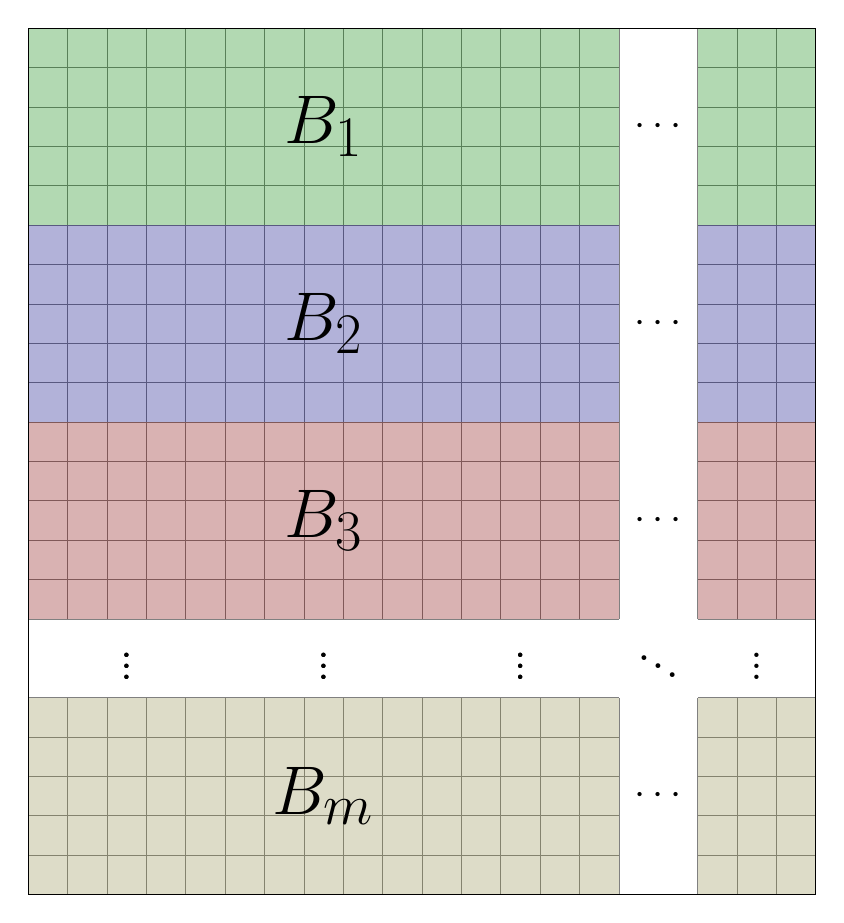
\begin{tikzpicture}
			\draw[step=5mm,gray,very thin] (0,0) grid (7.5,7.5);
			
			\draw[step=5mm,gray,very thin] (0,0) grid (7.5,7.5);
			\draw[step=5mm,gray,very thin] (0,-3.5) grid (7.5,-1);
			
			\draw[step=5mm,gray,very thin] (8.49999,-3.5) grid (10,-1);
			\draw[step=5mm,gray,very thin] (8.49999,0) grid (10,7.5);
			
			\fill[yellow!50!black,opacity=0.3]   (0,-3.5) rectangle (7.5,-1);
			\fill[yellow!50!black,opacity=0.3]   (8.49999,-3.5) rectangle (10,-1);
			
			\fill[green!50!black,opacity=0.3] (0,7.5) rectangle (7.5,5);
			\fill[green!50!black,opacity=0.3] (8.49999,7.5) rectangle (10,5);
			
			\fill[blue!50!black,opacity=0.3]  (0,5) rectangle (7.5,2.5);
			\fill[blue!50!black,opacity=0.3]  (8.49999,5) rectangle (10,2.5);
			
			\fill[red!50!black,opacity=0.3]   (0,2.5) rectangle (7.5,0);
			\fill[red!50!black,opacity=0.3]   (8.49999,2.5) rectangle (10,0);
			
			\node at (8, -2.25) {\bf \Large $\cdots$};
			\node at (8, 1.25) {\bf \Large $\cdots$};
			\node at (8, 3.75) {\bf \Large $\cdots$};
			\node at (8, 6.25) {\bf \Large $\cdots$};
			
			\node at (1.25, -0.5) {\bf $\vdots$};
			\node at (3.75, -0.5) {\bf $\vdots$};
			\node at (6.25, -0.5) {\bf $\vdots$};
			\node at (9.25, -0.5) {\bf $\vdots$};
			
			\node at (8, -0.5) {\bf \large $\ddots$};
			
			\node at (1.25, -0.5) {\bf $\vdots$};
			\node at (3.75, -0.5) {\bf $\vdots$};
			\node at (6.25, -0.5) {\bf $\vdots$};
			
			\node at (3.75, -2.25) {\Huge \bf $B_{m}$};
			\node at (3.75, 1.25) {\Huge \bf $B_3$};
			\node at (3.75, 3.75) {\Huge \bf $B_2$};
			\node at (3.75, 6.25) {\Huge \bf $B_1$};
			
			\draw[black] (0,7.5) rectangle (10,-3.5);
			\end{tikzpicture}
		}
	\end{figure}
\end{frame}

\begin{frame}
	\frametitle{Generic block algorithm}
	\begin{algorithm}[H]
		\DontPrintSemicolon
		\For {each processing element $P_{l}$} {
			\For {$i = 1, 2, \ldots$ until convergence} {
				Pick a block $j \in \{1, 2, \ldots, m\}$ {\em{\underline{somehow}}} \; 
				Read the corresponding entries of $A, x, b$ \;
				Perform Jacobi or Gauss-Seidel relaxations for all equations in block $j$ \;
				Update the data for block $j$ \;
			}
		}
	\end{algorithm}
	\begin{itemize}
		\item The way that each processor selects the block it works on can alter convergence
		\item Before going into block selection strategies, first a brief aside regarding synchronous and asynchronous updates
	\end{itemize}
\end{frame}


\begin{frame}
	\frametitle{Fixed Point Methods}
	\begin{itemize}
		\item The solvers focused on here can all be expressed as fixed point iterations of the form
			\begin{equation}
				x = G(x)
			\end{equation}
		\item In terms of parallelism for these methods:
		\begin{itemize}
			\item Each component (or block of components) can be treated as a task and assigned to a single processor
			\item Each processor {\em should} be able to complete its current task without receiving new information from other processors 
		\end{itemize}
	\end{itemize}
\end{frame}

\begin{frame}
	\frametitle{Residual data for finite-difference of 2D Laplacian}
	\begin{figure}[H]
		\centering
		\subfloat[Unsorted residuals]{\includegraphics[width=0.45\textwidth]{images/init_resids_10x10.pdf}}
		\subfloat[Sorted residuals]{\includegraphics[width=0.45\textwidth]{images/init_resids_10x10_sorted.pdf}}
		\caption{Initial component residuals ($r_i / \max (r_i)$).}
		\label{fig:initial-residuals-laplacian}
	\end{figure}
\end{frame}

\begin{frame}
	\frametitle{Ranked residual data for finite-difference of 2D Laplacian}
	\begin{figure}[H]
		\centering
		\subfloat[Sorted Residuals, exponential distributions]{\includegraphics[width=0.45\textwidth]{images/exp_dist_overlay_10iter.pdf}}
		\subfloat[Sorted Residuals, triangular distributions]{\includegraphics[width=0.45\textwidth]{images/normal_dist_overlay_10iter.pdf}}
	\end{figure}
	\begin{itemize}
		\item Need to balance computational cost associated with generating a ranked list and fitting a distribution with the benefit in doing so
	\end{itemize}
\end{frame}

\begin{frame}
	\frametitle{Solver data (Laplacian)}
	\begin{figure}[H]
		\centering
		\subfloat[2D problem (5-pt stencil, $10\times 10$ grid)]{\includegraphics[width=0.45\textwidth]{images/res_10x10.pdf}}
		\subfloat[3D problem (27-pt stencil, $10 \times 10 \times 10$ grid)]{\includegraphics[width=0.45\textwidth]{images/res_3D_10x10x10.pdf}}
		\caption{Residual ($r / r_0$) progression for the first 10,000 iterations of four stationary methods solving the 2D (a) and 3D (b) Laplacian.}
	\end{figure}
\end{frame}

\begin{frame}
	\frametitle{Moving forward I}
	\begin{itemize}
		\item Proving convergence as a per iteration reduction in the expected error
		\begin{itemize}
			\item Existing work proves relations such as (for synchronous, uniformly randomized, block Gauss-Seidel):
			\begin{equation}
			\mathbb{E}[\Vert x^{(k)} - x^* \Vert ] \leq \left( 1 - \frac{\beta (2 - \beta) \lambda_{min}}{n}\right)^k \Vert x^{(0)} - x^* \Vert^2_A
			\end{equation}
		\end{itemize}
		\item Dealing with the distributed memory environment
			\begin{itemize}
				\item Most approaches to this problem analyze and experiment with shared memory environments (e.g. a single workstation/GPU)
				\item Extending to the distributed environment is non-trivial
			\end{itemize}
		\item Incorporating new solvers into more complex existing routines
	\end{itemize}
\end{frame}
 
\begin{frame}
	\frametitle{Moving forward II}
	\begin{itemize}
		\item Experimenting with different distributions (still chosen beforehand) and ranking methods and periodicities
		\item Dynamically fitting the residual or difference data with an evolving probability distribution
		\item Investigating the impact that different problems have
			\begin{itemize}
				\item If all blocks have equal contribution to the residual, using a non-uniform distribution has no benefit
				\item Are there problems that some approaches can handle that others can't?
			\end{itemize}
		\item Look into the performance inside of more complicated ``real world'' applications
			\begin{itemize}
				\item Do these small differences even matter?
			\end{itemize}
	\end{itemize}
\end{frame}

%\section{A (slightly more) formal approach}
%
%\begin{frame}
%	\frametitle{Notation (following Griebel and Oswald, 2012)}
%	\begin{itemize}
%		\item Let:
%			\begin{itemize}
%				\item $V$ be a separable Hilbert space
%				\item $a(\cdot, \cdot)$ be a continuous symmetric positive definite bilinear form on $V$
%				\item $F$ be a bounded linear functional on $V$
%				\item $V_a$ represent the Hilbert space with scalar product given by the bilinear form $a(\cdot, \cdot)$ 
%			\end{itemize}
%		\item The problem becomes a variational problem, (iteratively) find $u \in V$ such that
%			\begin{equation}
%				a(u,v) = F(v) 
%			\end{equation}
%			 for all $v \in V$
%	\end{itemize}
%\end{frame}
%
%\begin{frame}
%	\frametitle{Notation (continued)}
%	\begin{itemize}
%		\item The iteration from before becomes an iterative subspace correction scheme
%		\item Let $V_a$ be represented by a finite collection of Hilbert spaces, $V_{a_i}$, along with inner products $a_i(\cdot, \cdot)$, and bounded linear operators, $R_i: V_{a_i} \rightarrow V_a$ as follows:
%			\begin{equation}
%				V_a = \sum_{i=1}^N R_i V_{a_i} = \lbrace v = \sum_{i=1}^N R_i v_i : v_i \in V_{a_i}, i = 1, \ldots, N \rbrace
%			\end{equation}
%		\item As before, the subspaces don't have to be disjoint but they can be thought of that way
%	\end{itemize}
%\end{frame}
%
%\begin{frame}
%	\frametitle{...and further}
%	\begin{itemize}
%		\item There are upper bounds on the $R_i$ operators
%			\begin{equation}
%				a(R_i v_i, R_i v_i) \leq \gamma_i a_i (v_i, v_i)
%			\end{equation}
%		\item Define operators $T_i: V_a \rightarrow V_{a_i}$
%			\begin{equation}
%				a_i(T_i v, v_i) = a(v, R_i v_i)
%			\end{equation}
%		\item Define the error at each iteration (in order to compute a residual) as
%			\begin{equation}
%				e^{(k)} = u - u^{(k)}
%			\end{equation}
%			which can be solved since the variational problem at each iteration can be solved without knowledge of $u$
%	\end{itemize}
%\end{frame}
%
%\begin{frame}
%	\frametitle{Bringing it back}
%	\begin{itemize}
%		\item In terms of the block methods discussed earlier for solving $Ax = b$, where $A$ is SPD:
%			\begin{itemize}
%				\item $V = \mathbb{R}^n$
%				\item The space splitting is based on the coordinate vectors, $e_i$ (so each $V_{a_i}$ is a copy of $\mathbb{R}$)
%				\item $a(x,y) = y^T Ax$, $F(x) = b^T x$, and $a_i(x_i, y_i) = x_i y_i$
%				\item The operators $R_i$ go from $V_{a_i}$ to $V_a$ and can be defined by $R_i(x_i) = x_i e_i$
%				\item The bounds $\gamma_i$ are just there to ensure the iterate mapping is ``contractive''; setting them to the diagonal elements $a_{ii}$ is sufficient
%				\item The operators $T_i$ are defined by the variational problem (which is controlled by $a_i(\cdot,\cdot)$ and $a(\cdot,\cdot)$); here $T_i v = (Av)_i$
%			\end{itemize}
%	\end{itemize}
%\end{frame}
%
%\begin{frame}
%	\frametitle{General algorithm}
%	\begin{algorithm}[H]
%		\DontPrintSemicolon
%		\KwIn{Space splitting-$V_a$, operators $R_i, T_i$, initial guess $u^{(0)} \in V_a$, relaxation parameter $\beta$, bounds $\gamma_i$}
%		\For {$k = 1, 2, \ldots$ until convergence} {
%			Compute the residuals, $r_i^{(k)} = T_i e^{(k)}$ \;
%			Choose an index, $i^*$, associated with a desired subspace \;
%			Set $u^{(k)} = u^{(k-1)} + \frac{\beta}{\gamma_i} R_{i^*} r_{i^*}^{(k-1)}$ \;
%		}
%	\end{algorithm}
%\end{frame}

\section{Summary \& Path Forward}

\begin{frame}
	\frametitle{Summary \& Path Forward}
	\begin{itemize}
		\item While linear solvers are prevalent throughout science and engineering, the idea of using weighted randomization could find uses in other key areas
		\item Example: convex optimization 
			\begin{itemize}
				\item stochastic gradient descent, and variants thereof
				\item current research mainly focuses on uniformly selecting components, but some studies have examined using a Southwell-like approach with some success
					\begin{itemize}
						\item using weighted randomization may allow a blend between the two approaches
					\end{itemize}
			\end{itemize}
	\end{itemize}
\end{frame}










\end{document}